%% Copernicus Publications Manuscript Preparation Template for LaTeX Submissions
%% ---------------------------------
%% This template should be used for copernicus.cls
%% The class file and some style files are bundled in the Copernicus Latex Package which can be downloaded from the different journal webpages.
%% For further assistance please contact the Copernicus Publications at: publications@copernicus.org
%% http://publications.copernicus.org


%% Please use the following documentclass and Journal Abbreviations for Discussion Papers and Final Revised Papers.


%% 2-Column Papers and Discussion Papers
\documentclass[hess, manuscript]{copernicus}
%\documentclass[hess]{copernicus}

%% Journal Abbreviations (Please use the same for Discussion Papers and Final Revised Papers)
% Hydrology and Earth System Sciences (hess)

\usepackage[utf8]{inputenc}


%TODO: english editing
%TODO: perspective Obled: MTW without precip -> indicator


\begin{document}

\linenumbers

\title{The Analog Method for Precipitation Prediction: Finding Better Analog Situations at a Sub-Daily Time Step}


\Author[1,2]{Pascal}{Horton}
\Author[3]{Charles}{Obled}
\Author[1]{Michel}{Jaboyedoff}

\affil[1]{University of Lausanne, Institute of Earth Sciences, Lausanne, Switzerland}
\affil[2]{University of Bern, Oeschger Centre for Climate Change Research, Institute of Geography, Bern, Switzerland}
\affil[3]{Universit\'{e} de Grenoble-Alpes, LTHE, Grenoble, France}



\runningtitle{Finding Better Analog Situations at a Sub-Daily Time Step}

\runningauthor{P. Horton et al.}

\correspondence{Pascal Horton (pascal.horton@alumnil.unil.ch)}



\received{}
\pubdiscuss{} %% only important for two-stage journals
\revised{}
\accepted{}
\published{}

%% These dates will be inserted by Copernicus Publications during the typesetting process.


\firstpage{1}

\maketitle



\begin{abstract}
The Analog Method (AM) aims at predicting local weather variables (predictands), such as precipitation, by means of a statistical relationship with predictors at a synoptic scale. The analogy is generally first assessed on gradients of geopotential fields, in order to sample days with a similar atmospheric circulation. Other predictors, such as moisture variables, can also be added in a successive level of analogy.

The search for candidate situations, for a given target day, is usually undertaken by comparing the state of the atmosphere at fixed hours of the day, for both the target day and the candidate analogs. The main reason is the use of daily precipitation time series, due to the length of their available archives, and the unavailability of equivalent archives at a finer time step. However, it is unlikely for the best analogy to happen at the very same hour, as it may occur at a different time of the day. In order to assess the potential of finding better analogs at a different hour, a moving time window (MTW) has been introduced on a reduced archive of hourly precipitation totals.

The MTW resulted in a better analogy in terms of the atmospheric circulation, with improved values of the analogy criterion on the whole distribution of analog dates. The improvement was found to grow with the analog rank due to an accumulation of more similar situations in the selection. A seasonal effect has also been identified, with larger improvements in winter than in summer, supposedly due to stronger diurnal cycles in summer, which favor predictors at the same hour for the target and analog days.

The impact of the MTW on the prediction skill has been assessed by means of a sub-daily precipitation series transformed into moving 24~h-totals at a 6-hourly time step. The prediction skill was found to be improved by the MTW, and even more after recalibrating the AM parameters. Moreover, the improvement was greater for days with heavy precipitation, which are generally related to more dynamic atmospheric situations, where timing is more specific, and which are less present in the archive. 

However, the MTW requires sub-daily precipitation time series, which are generally available on a shorter period than daily precipitation archives. Thus, two simple temporal disaggregation methods were assessed in order to make longer archives usable with the MTW. The assessed approaches were not successful, which emphasized the need to use time series with an appropriate chronology. These should be available in a near future, either by means of growing archives of measurements, or by the establishment of regional precipitation reanalyzes. Then, the use of a MTW in AMs can be considered for any application, and in any context, let it be operational forecasting or climate-related studies.

\end{abstract}



\introduction  %% \introduction[modified heading if necessary]
\label{sec:introduction}

Analog methods (AMs) are based on the hypothesis that two relatively similar synoptic situations may produce similar local effects \citep{Lorenz1956, Lorenz1969}. They are part of statistical downscaling methods \citep{Maraun2010}, and consist in finding past situations that are similar, in terms of the atmospheric circulation or other synoptic predictors, to the target day of interest. Then, the local weather variables of interest (predictand) that were observed at the analog dates are used to construct a probabilistic prediction for the target day \citep{Duband1970, Zorita1999}. Multiple variations of the method exist \citep[a non-exhaustive listing can be found in][]{BenDaoud2016}. AMs are used for operational precipitation forecasting, either in the context of flood forecasting or hydropower production \citep[e.g.,][]{Guilbaud1997, Bontron2005, Hamill2006, Desaint2008a, GarciaHernandez2009b, Bliefernicht2010, Marty2010, Marty2012, Horton2012, Obled2014, Hamill2015, BenDaoud2016}, as well as precipitation downscaling in a climate perspective \citep[e.g.,][]{Radanovics2013, Chardon2014, Dayon2015}. Other applications focus on temperatures \citep{Radinovic1975, Woodcock1980, Kruizinga1983, DelleMonache2013, Caillouet2016}, wind \citep{Gordon1987, DelleMonache2013, DelleMonache2011, Vanvyve2015, Alessandrini2015, Junk2015, Junk2015c}, solar power \citep{Alessandrini2015a, Bessa2015}, snow avalanches \citep{Obled1980, Bolognesi1993}, insolation \citep{Bois1981}, and the trajectories of tropical cyclones \citep{Keenan1981, Sievers2000, Fraedrich2003}.

The spatial transferability of the method is analyzed in \citet{Chardon2014}. A great advantage of AMs is that they create realistic precipitation patterns, as they are based on observed situations, with consistent spatial distribution, as long as the analog dates chosen for a region are the same. The temporal transferability has also been the topic of recent studies, may it be for past or future climates \citep{Dayon2015, Caillouet2016}.

\citet{Ruosteenoja1988} and \citet{Vandendool1994} have analyzed the influence of the archive length on the quality of the analogy. They highlight a three-way relationship between the quality of the analogy, the archive length and the size of the spatial domain (or degrees of freedom): errors increase with a bigger domain, but decrease with a longer archive. They demonstrate that it is not possible to find good analogs on the whole northern hemisphere with a 100 years archive (and even for much higher orders of magnitude). For that reason, smaller spatial windows are always considered to search for analogs, and the archive length is maximized. 

Thus, due to the availability of long precipitation archives at a daily time step that have no equivalent at a finer resolution, AMs are usually implemented on a daily basis (see references above). Therefore, the analog situations are assessed by comparing predictors at fixed hours of the day. However, it can be expected that the analogy of the synoptic situations does not occur systematically at the same time of the day, and that better candidates can be found by shifting to a different hour. On this assumption, a moving time window (MTW) was introduced to allow searching for candidates at different hours of the day. Previous tests showed the benefit, in terms of analogy criterion values, of searching for analog synoptic situations at a finer time step, but without assessing the impact on the prediction skills \citep{Finet2008}.

The MTW allows finding analog situations at different hours of the day, which can also be seen as an inflation of the archive length. However, despite having $x$ time more candidate situations, the quantity of new information is not expected to be as important as a $x$ time longer archive, due to significant correlation between successive situations within the same day. Nevertheless, if the MTW can improve the prediction skill of the AM, it means that it does extract new information from the archive. Thus, if the reduction of the archive length necessary to the MTW, due to the reduced availability of sub-daily precipitation time series, is expected to decrease the AM performance, the archive inflation brought by the MTW is expected to contribute to an increase in performance.

Other possibilities exist in order to increase the prediction skill of AMs. A classical approach is to add new predictors or new successive levels of analogy \citep[see e.g.][]{Horton2012a, BenDaoud2016, Caillouet2016}. AMs can also be combined with other methods \citep[see e.g.][]{Chardon2014}. Another possibility is to use a global optimization technique, such as genetic algorithms, in order to better optimize the method and to add new parameters \citep{Horton2016}. However, the MTW technique is not in competition with other approaches, but can be combined with these. Indeed, as most of them rely on the atmospheric circulation in the first level of analogy, the application of a MTW should lead to similar conclusions.

Section \ref{sec:data_methods} presents the context of the study as well as data and methods, including the proposed MTW technique. The impact of the reduction of the archive and the improvements brought by the MTW are assessed in Sect. \ref{sec:results}. The benefit of introducing a MTW was assessed first in regards to the analogy criterion improvement (Sect. \ref{sec:influence_criteria}), and then in terms of precipitation prediction skill (Sect. \ref{sec:influence_scores}). Finally, the results are discussed in Sect. \ref{sec:discussion} and the conclusions are found in Sect. \ref{sec:conclusions}.


\section{Data and methods}
\label{sec:data_methods}

\subsection{Study area and data}
\label{sec:data}

The study area is the upper Rh\^{o}ne catchment in Switzerland. Precipitation time series come from 6 automatic weather stations, namely Ulrichen, Zermatt, Visp, Montana, Sion and Aigle (Fig. \ref{fig:map}), which are subject to various meteorological influences \citep{Horton2012}. The data were available at an hourly time step on 25~years (1982 to 2007), and were also obtained at a daily time step (from 6~h~UTC to 6~h~UTC the next day) on 47~years (1961 to 2008). Due to the low density of weather stations with high temporal resolution and long archives, no spatially aggregated rainfall was processed. The results will thereafter be presented arbitrarily for the Ulrichen station, but were equivalent for all stations.

Synoptic-scale variables, used as predictors, were extracted from the NCEP/NCAR reanalysis I dataset \citep{Kalnay1996} with a 6-hourly temporal resolution, 17 pressure levels, and a spatial resolution of 2.5\degree. This dataset is now relatively old, but it is not expected to affect the conclusions of the present study (see discussion in Sect. \ref{sec:old_reanalysis}).


\subsection{The considered analog method}
\label{sec:analog_method}

The first considered AM is based on the analogy of the atmospheric circulation only \citep[Table \ref{table:method_2Z},][]{Obled2002, Bontron2005, Marty2012}. Searching for analog situations to a target day starts by a seasonal stratification through a preselection step of the potential candidates for analogy. The restriction is here a search for analog days within a 4 months window centered on the target date, for every year of the archive. Then, the similarity of the atmospheric circulation of the target date with every day of the preselection is assessed by processing the \citet{Teweles1954} score (S1), which is a comparison of gradients, on geopotential heights over a certain spatial window and at certain hours. The smaller the S1 values, the more similar the pressure fields.

The predictor variables, extracted from reanalysis datasets, are considered at different hours of the day. Based on \citet{Bontron2005}, geopotential heights are thus compared at 1000~hPa (Z1000) at 12~h~UTC and 500~hPa (Z500) at 24~h~UTC. The time of the day at which the predictors are selected is found by \citet{Bontron2004} to have a significant influence.

Then, $N_{1}$ dates with the lowest values of S1 are considered as analogs to the target day, $N_{1}$ being a parameter to calibrate (see Sect. \ref{sec:calibration}). Finally, the daily observed precipitation amount of the corresponding dates provide the empirical conditional distribution considered as the probabilistic prediction for the target day. This method will be named 2Z further on.

The second reference method (2Z-2MI, Table \ref{table:method_2Z-2MI}) adds a subsequent level of analogy on moisture variables, compared by means of the root-mean-square error (RMSE). The additional predictor is a moisture index made of the product of the total precipitable water (TPW) with the relative humidity at 850~hPa (RH850) \citep{Bontron2004}. When adding a second level of analogy, $N_{2}$ dates are subsampled from the $N_{1}$ analogs on the atmospheric circulation, to end up with a smaller number of analog situations. When a second level of analogy is added, a higher number of $N_{1}$ analogs is kept on the first level.

More complex AMs exist, with additional predictors \citep[see e.g.][]{Horton2012a, BenDaoud2016, Caillouet2016}. The MTW can also be applied on these, as they generally rely on a similarity of the atmospheric circulation in the first level of analogy, but it is easier to interpret the impact of the MTW on more basic methods.


\subsection{Performance score}
\label{sec:performance}

In order to assess the performance of AMs, the continuous ranked probability score \citep[CRPS,][]{Brown1974, Matheson1976, Hersbach2000} is often employed \citep[see, e.g.,][]{Bontron2004, Bontron2005, BenDaoud2008, Horton2012, Marty2012, Radanovics2013, Chardon2014, Junk2015, BenDaoud2016, Caillouet2016}. It allows evaluating the predicted cumulative distribution functions $F(y)$, for example of the precipitation values $y$ from analog situations, compared to the observed value $y^{0}$. The better the prediction, the smaller the score. It is defined as follows:

\begin{equation}
\label{eq:CRPS}
S_{\text{CRP}} = \int_{-\infty}^{+\infty} \left[ F(y)-\text{H}(y-y^{0})\right]^{2} \text{d}y ,  
\end{equation}
where $\text{H}(y-y^{0})$ is the Heaviside function that is null when $y-y^{0}<0$, and has the value 1 otherwise.

In order to compare the value of the score in regard to a reference, one often considers its skill score expression, and use the climatological distribution (i.e. the distribution of all precipitation values from the corresponding archive) as the reference. The continuous ranked probability skill score (CRPSS) is thus defined as follows:

\begin{equation}
\label{eq:CRPSS}
S_{\text{SCRP}} = \frac{S_{\text{CRP}}-S_{\text{CRP}}^{r}}{S_{\text{CRP}}^{p}-S_{\text{CRP}}^{r}} = 1-\frac{S_{\text{CRP}}}{S_{\text{CRP}}^{r}}
\end{equation}
where $S_{\text{CRP}}^{r}$ is the $S_{\text{CRP}}$ value for the reference (climatological distribution) and $S_{\text{CRP}}^{p}$ would be the one for a perfect prediction (which implies $S_{\text{CRP}}^{p}~=~0$). A better prediction is characterized by an increase in CRPSS: $S_{\text{SCRP}}~=~1$ for a perfect prediction, and $S_{\text{SCRP}}~<~0$ for a prediction with a lower skill than the reference.


\subsection{The moving time window (MTW) approach}
\label{sec:mtw}

The moving time window (MTW) technique aims at finding better analog situations at different hours of the day rather than comparing the predictors at fixed hours. Thus, instead of looking for analogs at a 24-hourly time step, they are sought at the time step matching the predictor temporal resolution, which is here 6-hourly (Fig. \ref{fig:principle}).

The target situations and their corresponding observed precipitation values do not change, because the prediction is still established on a daily basis, for a fixed period of the target day (6~h~UTC to 6~h~UTC the next day), as before. The difference is that the candidates are 4~times more numerous (even though they are not fully independent). No constraint was added in order to restrict the selection of multiple analogs within the same candidate dates.

In order to assess the benefit of searching analog situations at a sub-daily time step, an appropriate precipitation series is required. On the basis of high temporal resolution time series (Sect. \ref{sec:data}), 24~h-totals were processed, but at a 6-hourly time step, by means of a moving 24~h-total.  As sub-daily precipitation time series are available on a shorter period than daily ones, the loss of performance resulting from a reduction of a 47~years archive (1961 to 2008) to 25~years (1982 to 2007) needs to be assessed.


\subsection{Reconstruction of a longer precipitation archive}
\label{sec:reconstruction}

It would be profitable to be able to apply the MTW to a longer archive (here, 1961 to 2008), rather than being limited to the reduced period corresponding to the sub-daily precipitation data (cf. previous section). Thus, in order to reconstruct a longer archive of moving 24~h-totals, two simple disaggregation approaches of the daily precipitation time series were assessed.

The first technique was a proportional distribution, where the observed daily precipitations were considered constant during the measuring period (6~h~UTC to 6~h~UTC the next day). It then consisted in allocating proportional parts of the original daily time series into a new moving average of 24~h-totals (Fig. \ref{fig:illustration_disaggregation}). 

The second approach aimed at getting closer to the chronology of the actual precipitation by relying on some informative variables during the reconstruction procedure. Data from the NCEP/NCAR reanalysis 1 (Sect. \ref{sec:data}) were used in this perspective, despite their rough resolution. Precipitable water and relative humidity (at 1000~hPa, 925~hPa or 850~hPa) were assessed at the four points surrounding the catchment, and by allowing a time lapse between both series in order to take into account the significant distance separating the weather stations and the reanalysis grid point. The best proxy variable was identified by means of a correlation analyses (on non-zero values) with the 6-hourly precipitation time series on the period 1982-2007. Then, once the best proxy has been selected, its temporal profile was used in order to disaggregate the daily precipitation time series.


\subsection{Calibration of the analog method}
\label{sec:calibration}

The semi-automatic sequential procedure elaborated by \citet{Bontron2004} was used to calibrate the AM \cite[see also ][]{Radanovics2013, BenDaoud2016}. The analogy levels (e.g. the atmospheric circulation or moisture index) are calibrated sequentially. The parameters calibrated by this approach, for every level of analogy, are the spatial windows on which the predictors are compared and the number of analogs. The procedure consists of the following steps \citep{Bontron2004}:

\begin{enumerate}
	\item Manual selection of the following parameters:
	\begin{enumerate}
		\item meteorological variable (e.g. geopotential height, temperature, relative humidity, etc.),
		\item pressure level (e.g. 500 hPa, ...),
		\item temporal window (hour of the day \textendash\ e.g. 6, or 12~h~UTC),
		\item initial analog numbers (e.g. $N_{1}=50$).
	\end{enumerate}
	
	\item For every level of analogy:
	\begin{enumerate}
		\item Identification of the most skilled unitary cell (1~point for moisture variables and 4 for the geopotential height when using the S1 criterion) over a large domain. Every point (or cell) of the full domain is assessed on all predictors of the level of analogy, jointly (consisting generally of the same variable, but on different pressure levels and at different hours).
		\item From this most skilled point, the spatial window is expanded by successive iterations in the direction of greater performance gain. The spatial window grows up by repeating the previous steps, until no improvement is reached.
		\item The number of analog situations is then reconsidered and optimized for the current level of analogy.
	\end{enumerate}
	\item A new level of analogy can then be added, based on other variables (such as the moisture index) at chosen pressure levels and hours of the day. The number of analogs for the next level of analogy is initiated at a chosen value. Then, the procedure starts again from step (2) for the new level. The parameters calibrated on the previous analog levels are fixed and do not change. 
	\item Finally, the numbers of analogs for the different levels of analogy are re-assessed. This is done iteratively by varying the number of analogs of each level in a systematic way.
\end{enumerate}

The calibration is thus done in successive steps, on a limited number of parameters. Previously calibrated parameters are generally not reassessed (except for the number of analogs). More advanced techniques, such as using genetic algorithms \citep{Horton2016}, exist, but are out of the scope of the present study.


\section{Results}
\label{sec:results}

\subsection{Consequences of the archive reduction}
\label{sec:archive_reduction}

The performance loss resulting from the reduction of a 47~years archive (1961 to 2008, corresponding to the daily time series) to 25~years (1982 to 2007, corresponding to the hourly time series, see Sect. \ref{sec:mtw}) was assessed with the original method, without MTW. Both 2Z (Table \ref{table:method_2Z}) and 2Z-2MI (Table \ref{table:method_2Z-2MI}) methods were considered. The AM parameters were calibrated on the original archive (see resulting analog numbers in Tables \ref{table:analog_nb}) and were used thereafter.

The impact of the archive reduction can be seen in Fig. \ref{fig:plots_CRPSS_2Z} for the 2Z method and in Fig. \ref{fig:plots_CRPSS_2Z-2MI} for the 2Z-2MI method. As expected, a loss of performance could be observed for each station, except for that of Aigle, which seemed relatively indifferent to this change. This loss was globally significant, with up to -1.89 points for Visp and the 2Z method. 


\subsection{Influence on the analogy criterion}
\label{sec:influence_criteria}

\subsubsection{Changes in the atmospheric circulation analogy}
\label{sec:perf_2Z}

When searching for analogs in the first level of analogy, such as on the geopotential heights in the 2Z method (Sect. \ref{sec:analog_method}), there are 4 times more candidates (even though not fully independent) with the MTW than before (Sect. \ref{sec:mtw}). Figure \ref{fig:changes_S1_analogs} shows the changes in the distributions of the analogy criterion (S1) for the $1^{st}$, $5^{th}$, $20^{th}$ and $40^{th}$ analog rank at the Ulrichen station on the whole calibration period (1961-2008 -- the full period could be used here, as precipitation were not considered at this stage), due to introduction of the MTW. The shape of the distributions of the conventional approach and the MTW were found to be similar, but the values of the analogy criterion were reduced (shifted to the left), and were therefore better. For analogs with higher ranks (e.g. $20^{th}$ or $40^{th}$), the difference between the two distributions was larger than for the first ranks, which means that the improvement increased with the rank of the analogs. 

The improvements of the S1 criterion with the rank of the analogs are summarized in Fig. \ref{fig:changes_S1}, which shows (top) quantiles of the S1 criterion for the conventional method and the MTW, and (bottom) quantiles of the relative reduction (meaning improvement) due to the MTW. This confirms that all quantiles were similarly reduced (S1 distributions keep their shape), and that this improvement was constantly increasing from the first to the last analog (Fig. \ref{fig:changes_S1} bottom).


\subsubsection{Changes per precipitation classes}
\label{sec:influence_precip}

The impact of the MTW on the analogy criterion has been analyzed per precipitation classes (for the target day). The results are summarized in Fig. \ref{fig:changes_S1_precip_threshold} by the median reduction of S1 for days with precipitation (organized into classes) between two thresholds. The number of cases per class being reduced, the curves are not as smooth as in previous analyzes. It is nevertheless clear that the improvement were more important on days with higher precipitation. Once again, the results for the other stations were similar.


\subsubsection{Changes per season}
\label{sec:seasonal_effect}

Atmospheric dynamics varies greatly from one season to another, which reflects on the performance of the AM that is generally lower between June and August \citep{Bliefernicht2010}. The effect of the MTW on the S1 criterion per season is presented in Fig. \ref{fig:changes_S1_seasons}. Differences between the seasons were substantial, with greater improvements for winter than summer. 


\subsubsection{Changes in the moisture analogy}
\label{sec:perf_2Z-2MI}

When adding the second level of analogy of the 2Z-2MI method (Table \ref{table:method_2Z-2MI}), the number of candidate situations did not increase, as they were conditioned by the $N_{1}$ previously selected analogs, but their dates have changed. In contrast to the AM on the atmospheric circulation only, both a reduction or an increase of the RMSE analogy criterion values were possible here with the MTW compared to the static approach. Indeed, Fig. \ref{fig:changes_RMSE} shows an almost insignificant improvement of the RMSE values. Unlike for the first level of analogy, the relative changes of the RMSE values were distributed relatively symmetrically around zero, with improvements and losses of the same amplitude.


\subsection{Impact on the prediction relevance}
\label{sec:influence_scores}

The new performance scores (CRPSS) are provided in Fig. \ref{fig:plots_CRPSS_2Z} and \ref{fig:plots_CRPSS_2Z-2MI} for the 2Z and 2Z-2MI methods respectively, on the reduced archive (1982--2007). The gains, relatively to the static approach on the same archive, ranged from 0.57 to 2.14 points for the 2Z method and from 1.53 to 2.20 points for the 2Z-2MI method. 


\subsubsection{Improvement per precipitation classes}
\label{sec:improvement_CRPSS_precip_threshold}

The S1 criterion was previously found to be improved to a greater extent for higher precipitation values (Sect. \ref{sec:influence_precip}). The changes in terms of performance scores were then also assessed per precipitation classes. Fig. \ref{fig:changes_CRPS_precip_threshold} synthesizes these differences for the Ulrichen station, the other stations having the same behavior. The performance score was improved for days with higher precipitation after the introduction of the MTW. On the contrary, non-rainy days and small precipitation values were not improved.


\subsubsection{Recalibration of the AM parameters}
\label{sec:recalibration}

The previous assessment of the performance improvement was established with the original parameters optimized with a fixed time window. However, one can assume that the introduction of the MTW might change the optimum value of some parameters. The calibration (see Sect. \ref{sec:calibration}) has then been reprocessed.

After recalibrating, changes in the AM parameters could be observed for both 2Z and 2Z-2MI methods. Among these, the zonal extent of the spatial windows of the circulation analogy decrease a bit (not shown). More significantly, the optimal number of analogs increased after introducing the MTW, of a considerable order of magnitude: 25~\% to 83~\% for the 2Z method, and 20~\% to 67~\% for the final selection of the 2Z-2MI method (Table \ref{table:analog_nb}). The number of analogs of the first analogy level of the 2Z-2MI method even reached three times its previous value for the Visp station. 

The values of the CRPSS scores for both methods (Fig. \ref{fig:plots_CRPSS_2Z} and \ref{fig:plots_CRPSS_2Z-2MI}) have significantly increased after recalibration. When analyzing the change in performance per precipitation classes, the results (not shown) were very similar to what was observed in Sect. \ref{sec:improvement_CRPSS_precip_threshold}, with a slight performance increase of small precipitation values that can be observed at the expense of higher amounts.


\subsection{Using a reconstructed archive}
\label{sec:reconstruction_results}

When using the first reconstructed time series (on the reduced period), based on the proportional distribution (see Sect. \ref{sec:reconstruction}), the AM performance was degraded and was even below the conventional method without MTW (Table \ref{table:disaggregation_proportional} to compare to Fig. \ref{fig:plots_CRPSS_2Z} and \ref{fig:plots_CRPSS_2Z-2MI}).

For the second approach, the synoptic proxy to use for the temporal disaggregation of the daily time series had to be identified first. The results are illustrated this time for the Zermatt station. Amongst the considered moisture variables (see Sect. \ref{sec:reconstruction}), the best proxy was the precipitable water at 45° N and 7.5° E, with a time offset of -6~h (Table \ref{table:proxy_correlations}). Table \ref{table:proxy_CRPSS} presents the CRPSS scores obtained by the disaggregated series using the proxy of precipitable water.


\section{Discussion}
\label{sec:discussion}


\subsection{Improvement of the selection of analog situations}

On the first level of analogy, the improvement of the S1 criterion (Fig. \ref{fig:changes_S1} bottom) started approximately at 5~\% for the first analog and reached more than 10~\% for the last one (Sect. \ref{sec:perf_2Z}). This increase of improvements with the analog rank can be explained by the accumulation of better analogs in the selection. The curve representing the minimum improvement is quickly slightly superior to zero, meaning that the criteria have been improved on most analog ranks for every day of the calibration period. All other stations had a similar improvement of the S1 criterion, both in terms of the distribution shape and amplitude. The introduction of the MTW allowed finding better analog situations in the first level of analogy, resulting in a selection of days with more similar atmospheric circulation.

When adding a second level of analogy on moisture variables, the criteria values (RMSE) were not improved by the MTW (Sect. \ref{sec:perf_2Z-2MI}), as the number of candidates was not higher (still the $N_{1}$ days selected in the first level of analogy). However, this result of a globally null improvement of the RMSE values does not mean that the 2Z-2MI method cannot be improved by the MTW. It means that after the selection of the analog situations in terms of the synoptic circulation, the new candidate dates did not allow to find better analogs in terms of moisture. However, the selected dates have changed in the first level of analogy, and thus also in the final selection, which did improve the prediction skill (Sect. \ref{sec:influence_scores}).


\subsection{Improvement of the precipitation prediction}

The MTW was found to improve the skill of the precipitation prediction for both the 2Z and 2Z-2MI methods (Fig. \ref{fig:plots_CRPSS_2Z} and \ref{fig:plots_CRPSS_2Z-2MI}, Sect. \ref{sec:influence_scores}). Moreover, it required no additional predictor. With the introduction of the MTW, the performance loss related to the reduction of the archive length was compensated. It was here of the same order of magnitude as if the length of the archive doubled. Note that despite the number of candidate situations being four times higher, the gains seem to be lower than for a quadrupled archive length. The likely reason is that an actual longer archive would contain more atmospheric situations that might have been less observed on a shorter period. Moreover, high correlations between sub-daily circulation patterns are expected. The MTW thus did not create four times more independent data, but the increase in information was nevertheless substantial. In this regards, a reanalysis dataset with a higher temporal resolution might not improve the performance significantly more than a 6-hourly dataset. On the other hand, reducing the MTW to a 12-hourly time step might reduce redundancy in the archive, but might also reduce the chance of finding better analog situations, as circulation patterns can evolve substantially in 12~hours.

Moreover, in a transient climate, an eventual non-stationarity of the link between predictors and precipitation might discard the relevance of analogs from far in the past, and thus increase the relevance of using a more recent and shorter archive rather than a long one. In such case, the archive inflation brought by the MTW is also relevant.

More complex methods with additional levels of analogy and more predictors do increase the performance score, and the MTW could also be applied in these situations, as it is likely to improve the analogy of the atmospheric circulation anyway. 

Both the analogy criteria (Sect. \ref{sec:influence_precip}) and the performance scores (Sect. \ref{sec:improvement_CRPSS_precip_threshold}) were improved to a greater extent for days with heavier precipitation. This is likely due to the fact that higher precipitation events are a consequence of atmospheric conditions with greater dynamics, such as weather disturbances, which have a well-marked temporal evolution. Indeed, the position of the driving elements such as the low-pressure center and the fronts change significantly during a day. Moreover, these situations are less numerous than anticyclonic situations, which makes it less likely to find very good analogs at the same time of the day. We can therefore expect to improve more significantly these situations with greater dynamics when introducing a MTW, as better matches to the target situation may be found. On the opposite, days with low dynamics of the atmospheric circulation, such as anticyclonic situations, will not be radically improved by the introduction of the MTW.

We just mentioned that the MTW improved the prediction of days with heavier precipitation. However, it will have no effect on the prediction of extreme events that were not yet observed, and therefore are not present in the archive. Extremes in AMs can be modeled e.g. by extrapolation of a truncated exponential or gamma distribution fitted on the analog values \citep{Obled2002}. Another possible approach is by combining AMs with other methods \citep[e.g.][]{Chardon2014}. However, this goes beyond the scope of the present study, as prediction of unobserved extremes are not modified by the MTW.


\subsection{Seasonal effect}

Section \ref{sec:seasonal_effect} and Fig. \ref{fig:changes_S1_seasons} revealed a difference of the improvement of the S1 criterion according to the season, with greater improvements for winter than summer. One hypothesis is that the diurnal effects of the summer months have an influence on the atmospheric circulation, at least in the lower layers. This effect is in phase with the daily cycle and good analogs are essentially found for the same hours.

An analysis of the selected hours for the geopotential predictor seems to confirm this assumption (Fig. \ref{fig:hours_selection_per_season}). It was found that the new choice of the temporal window in winter, when using the MTW approach, is well balanced between the 4 options. This means a change of 75\% of the analogs selection compared to the conventional approach. On the contrary, days in summer months had a preference for the initial temporal window (Z500 24~h \& Z1000 12~h), likely due to more pronounced diurnal effects which reduces the potential for improvement of the criteria. Other seasons were between these two extremes, which is consistent with their respective improvements. This seasonal effect was observed for each station in a very similar way, and generally even with a slightly larger amplitude than for Ulrichen.


\subsection{On the increase in number of analogs}

After the recalibration of the AMs with the MTW, the optimal analog numbers were significantly higher than in the original methods (see Sect. \ref{sec:recalibration} and Fig. \ref{table:analog_nb}). As we saw in Fig. \ref{fig:changes_S1}, the improvement of the S1 criterion grew along with the rank of the analog, which shows an accumulation of better analog situations in the distributions. It seems thus profitable to widen the selection of analogs in order to also keep some whose rank has increased, as they appear to be also relevant to predict precipitation values. The number of good analogs was thus globally increased.

A higher number of analogs generally means, with an archive of fixed length, a poorer analogy. Indeed, when the choice of the predictors or the parameters are improved, leading to a better prediction, the optimal number of analog situations decreases. However, when the length of the archive increases, the optimal number of analogs increases too, for a better performance, up to a certain threshold (\citealt{Bontron2004}, see also Fig. 7 of \citealt{Hamill2006a}). The observed increase in the number of analog situations with the MTW resulted in better performance skills for a given method, as it can be seen as an inflation of the archive. However, if new relevant predictors were added to the method, the number of analogs would then decrease.


\subsection{Why not just making a 6-hourly predictions ?}

One can question the interest of using moving daily totals when 6-hourly precipitation series can be predicted instead. A first reason is that the 6-hourly time series generated by the AM might not represent accurately the intra-daily precipitation distribution (results not shown). Also, sometimes one just does not need finer resolution than the daily time step, eventually using another disaggregation technique afterwards. Finally, when using a reconstructed precipitation archive, the errors in intra-day precipitation distributions have a lesser impact over 24~h daily totals.


\subsection{On the use of an old reanalysis dataset}
\label{sec:old_reanalysis}

The considered reanalysis dataset, which is the NCEP/NCAR reanalysis I \citep{Kalnay1996}, is relatively old and has a coarse resolution. Newer reanalysis dataset could have been used to achieve this study, and might have resulted in higher performance scores. However, \cite{BenDaoud2009} showed that the sensitivity of the method to the reanalysis dataset is rather small. This is particularly true for simple AMs that mainly rely on the atmospheric circulation, which is already well defined at a coarser resolution. That might not be the case of more elaborated methods relying on thermodynamic data. A comparative analysis of several reanalysis dataset within the AM is under work and will be the topic of a dedicated paper.

Moreover, one can assume that the gain observed here by introducing a MTW should also be found for a better reanalysis dataset. Indeed, a better dataset does not negatively influence the fact that one can find better analog situations at other hours of the day rather than at fixed hours.


\subsection{Relevance of the reconstructed precipitation archives}

The two simple methods assessed to reconstruct precipitation archives (Sect. \ref{sec:reconstruction}) did not result in valuable outputs (Sect. \ref{sec:reconstruction_results}). Indeed, the performance improvement brought by the MTW was lost due to a precipitation archive of poor quality. A slight improvement could be obtained for the second method relying on a proxy variable compared to the proportional distribution method, but it was still relatively small, and most of the benefit of the MTW was lost. A more recent reanalysis archive with more accurate moisture variables might produce better proxies.

These attempts to transpose the MTW on the total archive highlighted the importance of the actual rainfall chronology. The MTW is profitable, provided that the precipitation series are close to the observed one. Without precipitation series with an accurate sub-daily chronology, the introduction of a MTW does not improve the precipitation prediction.



\conclusions  %% \conclusions[modified heading if necessary]
\label{sec:conclusions}

AMs are most often based on a daily time step, due to the availability of long precipitation archives. However, it is unlikely that two analog synoptic situations, that evolve relatively quickly, would correspond optimally at the same hours of the day. It is thus probable that better matches can be found at another time, which can change the selection of the analogs dates.

As \citet{Finet2008} had previously shown, the introduction of a MTW allows finding better analog situations in terms of the atmospheric circulation. It has been here demonstrated that the improvement of the S1 criterion values was growing with the rank of the analog. This was due to the accumulation of better analogs within the predicted distributions.

The improvement of the circulation analogy was found to be more important for days with heavier precipitation, which are generally related to more dynamic atmospheric situations and are less frequent in the archive. These situations have more specific circulation patterns that are evolving more rapidly. Thus, a MTW was found to be of particular interest in this kind of situation, and benefits the prediction of heavier precipitation events.

A seasonal effect has been highlighted, as the MTW was more profitable for winter months than summer. The reason is likely that the diurnal cycle has a bigger effect in summer than in winter, which results in better analogs at the same time of the day. The preference for the same hours in summer has been demonstrated, whereas 75\% of the analog situations were selected at a different time in winter.

The impact of the MTW on the prediction skill has never been assessed before, due to the shortcoming of long precipitation series at a sub-daily time step. It was here assessed on a 25 years time series with a high temporal resolution. After the introduction of the MTW, the performance scores increased of the same order of magnitude as if the length of the archive doubled, in this case study.

The parameters were then calibrated again, using the MTW. Some parameters changed, the main difference being the number of analogs, which systematically and significantly increased compared to the original set. A wider selection of analog situations, containing those whose rank decreased, seemed profitable for the prediction performance. The number of good analogs was thus globally increased, in the same way as if the archive length increased. This change seems to benefit mainly the prediction of days with small precipitation totals.

The importance of the quality of the precipitation archive was also demonstrated, as too simplistic reconstructions of 6-hourly time series lead to a loss of all the improvement brought by the MTW. The precipitation prediction is improved only when the precipitation chronology is close to the accurate one. Attempts to reconstruct longer time series based on a simplistic proportional distribution or using meteorological variables from the NCEP reanalysis 1 dataset as proxy did not succeed. Other reanalysis datasets with more accurate moisture variables could eventually perform better.

Perspectives of using the MTW rely on the availability of long precipitation series at a sub-daily time step and with high accuracy. First, these archives of high temporal resolution precipitation data are increasing now with time. Another possible source of such archives is the establishment of precipitation reanalysis at a regional scale, or the use of reanalysis-driven RCMs (Regional Climate Models) or LAMs (Limited Area Models) on a long period. Even though outputs from these models might be biased or not accurate enough, information on the timing of the precipitation events could be useful in order to disaggregate stations time series. When precipitation data with accurate time distribution will be available, the use of a MTW in the AM can be considered for any application, and in any context, let it be operational forecasting or climate-related studies.



\begin{acknowledgements}
Thanks to the Swiss Federal Office for Environment (FOEV), the Roads and Water courses Service, Energy and Water Power Service of the Wallis Canton and the Water, Land and Sanitation Service of the Vaud Canton who financed the MINERVE (Mod\'{e}lisation des Intemp\'{e}ries de Nature Extr\^{e}me des Rivi\`{e}res Valaisannes et de leurs Effets) project which started this research. Thanks to Dominique B\'{e}rod for his support.

The fruitful collaboration with the Laboratoire d'Etude des Transferts en Hydrologie et Environnement of the Grenoble Institute of Technology (G-INP) was made possible thanks to the Herbette Foundation. 

NCEP reanalysis data provided by the NOAA/OAR/ESRL PSD, Boulder, Colorado, USA, from their Web site at http://www.esrl.noaa.gov/psd/. Precipitation time series provided by MeteoSwiss.

The authors would also like to acknowledge the work anonymous reviewers, which contributed to improving this paper. 
\end{acknowledgements}


%% REFERENCES

%% The reference list is compiled as follows:

\bibliographystyle{copernicus}
\bibliography{../_refs/4_articles-2016_HESS_moving-window}




\begin{figure}[htb]
	\begin{center}
		\includegraphics[width=8.3cm]{figures/figure_map.pdf}
	\end{center}
	\caption{Position of the 6 weather stations of interest (Ulrichen, Zermatt, Visp, Montana, Sion and Aigle) in the study area.}
	\label{fig:map}
\end{figure}

\begin{figure}[htb]
	\begin{center}
		
\includegraphics[width=8.3cm]{figures/illustration_moving_window.pdf}
	\end{center}
	\caption{Illustration of the principle of a moving time window. The larger horizontal bars represent the 24~h precipitation totals.}
	\label{fig:principle}
\end{figure}

\begin{figure}[htb]
	\begin{center}
		\includegraphics[width=8cm]{figures/illustration_disaggregation.pdf}
	\end{center}
	\caption{Illustration of the generation of 24~h-totals moving averages by means of a proportional distribution. The colours refer to the corresponding day of the daily time series.}
	\label{fig:illustration_disaggregation}
\end{figure}

\begin{figure}[htb]
	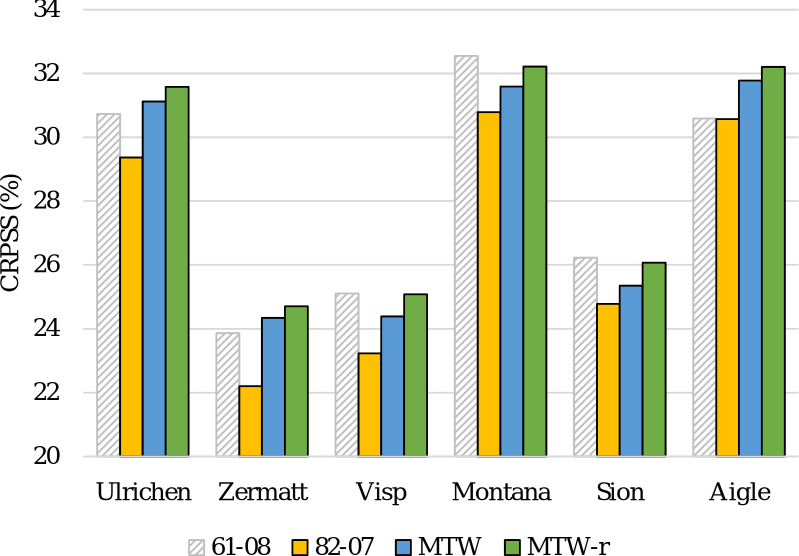
\includegraphics[width=8.3cm]{figures/plots_CRPSS_2Z.pdf}
	\caption{Performance score (CRPSS, \%) of the AM on the atmospheric circulation, at the different stations, for (dashed) the full archive, i.e. 1961-2008, (yellow) the reduced archive, i.e. 1982-2007, (blue) the introduction of the MTW on the reduced archive, and (green) the recalibrated parameters of the AM with the MTW.}
	\label{fig:plots_CRPSS_2Z}
\end{figure}

\begin{figure}[htb]
	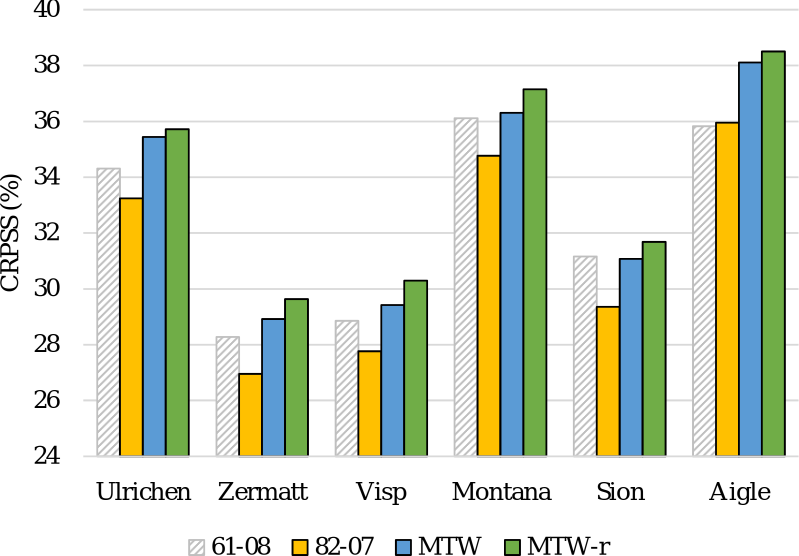
\includegraphics[width=8.3cm]{figures/plots_CRPSS_2Z-2MI.pdf}
	\caption{Same as Figure \ref{fig:plots_CRPSS_2Z}, but for the analog method with a second level on the moisture variables.}
	\label{fig:plots_CRPSS_2Z-2MI}
\end{figure}

\begin{figure*}[htb]
	\begin{center}
		\includegraphics[width=15cm]{figures/changes_S1_analogues.pdf}
	\end{center}
	\caption{Changes in the S1 criterion distributions, due to the MTW, of (a) the $1^{st}$, (b) $5^{th}$, (c) $20^{th}$ and (d) $40^{th}$ analog ranks for the Ulrichen station.}
	\label{fig:changes_S1_analogs}
\end{figure*}

\begin{figure}[htb]
	\begin{center}
		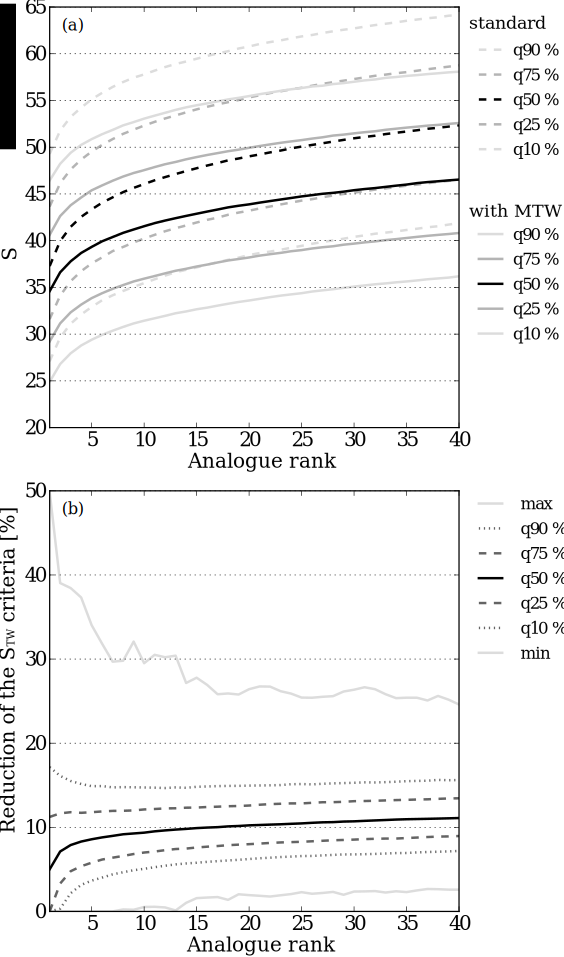
\includegraphics[width=8.2cm]{figures/changes_S1_value_and_gain.pdf}
	\end{center}
	\caption{Synthesis of the changes in the S1 criterion, due to the MTW, for the Ulrichen station, depending on the rank of the analog. (a) Quantiles of the S1 distributions with and without the MTW. (b) Quantiles of the relative improvements of the S1 criterion when using the MTW.}
	\label{fig:changes_S1}
\end{figure}

\begin{figure}[htb]
	\begin{center}
		\includegraphics[width=8.3cm]{figures/changes_S1_precip_threshold.pdf}
	\end{center}
	\caption{Distribution of the median improvements of the S1 criterion, due to the MTW, depending on precipitation thresholds at the Ulrichen station.}
	\label{fig:changes_S1_precip_threshold}
\end{figure}

\begin{figure}[htb]
	\begin{center}
		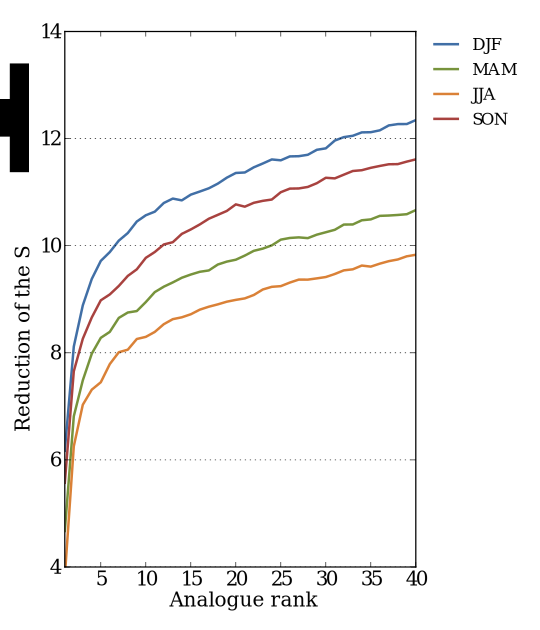
\includegraphics[width=7cm]{figures/changes_S1_seasons.pdf}
	\end{center}
	\caption{Seasonal effect on the median reduction of the S1 criterion for the Ulrichen station due to the MTW. DJF: winter, MAM: spring, JJA: summer SON: fall.}
	\label{fig:changes_S1_seasons}
\end{figure}

\begin{figure}[htb]
	\begin{center}
		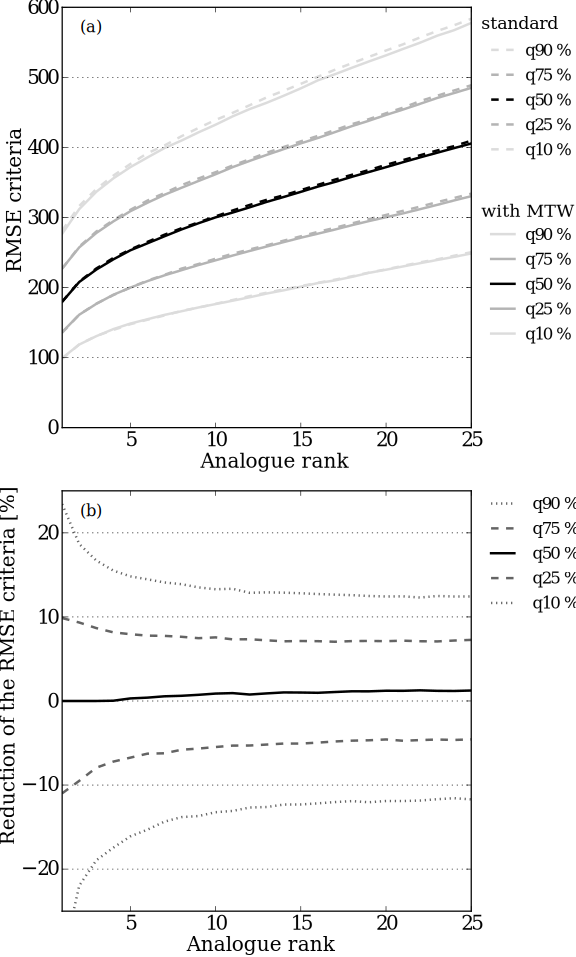
\includegraphics[width=8.1cm]{figures/changes_RMSE_value_and_gain.pdf}
	\end{center}
	\caption{Synthesis of the changes in the RMSE criterion, due to the MTW, for the Ulrichen station, depending on the rank of the analog. (a) Quantiles of the RMSE distributions with and without the MTW. (b) Quantiles of the relative improvements of the RMSE criterion when using the MTW.}
	\label{fig:changes_RMSE}
\end{figure}

\begin{figure}[htb]
	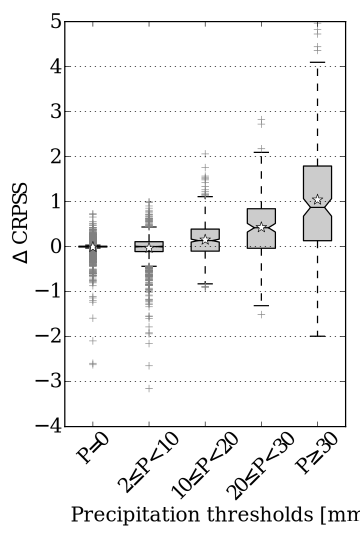
\includegraphics[width=5cm]{figures/changes_CRPS_precip_threshold.pdf}
	\caption{Differences of the CRPSS performance score, due to the introduction of the MTW, as a function of precipitation thresholds at the Ulrichen station. The stars represent averages.}
	\label{fig:changes_CRPS_precip_threshold}
\end{figure}

\begin{figure}[htb]
	\includegraphics[width=8.3cm]{figures/hours_selection_per_season.pdf}
	\caption{Distribution of the predictors hours in the selected analog dates depending on the season, for the Ulrichen station.}
	\label{fig:hours_selection_per_season}
\end{figure}


\clearpage


\begin{table}[htb]
	\caption{Parameters of the reference method on the atmospheric circulation (2Z). The first column is the level of analogy (0 for preselection), then comes the meteorological variable and its hour of observation (temporal window). The criterion used for the current level of analogy is then provided, as well as the number of analogs.}
	\footnotesize
	\begin{center}
		\begin{tabular}{ccccc}
			\hline
			Level & Variable & Hour & Criterion & Nb \\ 
			\hline 
			0 & \multicolumn{4}{l}{$\pm 60$ days around the target date} \\
			\hline 
			\multirow{2}{*}{1} & Z1000 & 12~h & \multirow{2}{*}{S1} & \multirow{2}{*}{$N_{1}$} \\
			& Z500 & 24~h & & \\ 
			\hline 
		\end{tabular} 
	\end{center}
	\label{table:method_2Z}
\end{table}

\begin{table}[htb]
	\caption{Parameters of the reference method with moisture variables (2Z-2MI). Same conventions as Table \ref{table:method_2Z}}
	\footnotesize
	\begin{center}
		\begin{tabular}{ccccc}
			\hline 
			Level & Variable & Hour & Criterion & Nb \\ 
			\hline 
			0 & \multicolumn{4}{l}{$\pm 60$ days around the target date} \\
			\hline 
			\multirow{2}{*}{1} & Z1000 & 12~h & \multirow{2}{*}{S1} & \multirow{2}{*}{$N_{1}$} \\
			& Z500 & 24~h & & \\ 
			\hline
			\multirow{2}{*}{2} & TPW * RH850 & 12~h & \multirow{2}{*}{RMSE} & \multirow{2}{*}{$N_{2}$} \\
			& TPW * RH850 & 24~h & & \\ 
			\hline 
		\end{tabular} 
	\end{center}
	\label{table:method_2Z-2MI}
\end{table}

\begin{table}[htb]
	\caption{Number of analogs (of the first and the second level of analogy, respectively $N_{1}$ and $N_{2}$) of the method based on the atmospheric circulation only (method 2Z), and the one with a second level of analogy on moisture variables (2Z-2MI), on the full archive (Standard) and after recalibration using the MTW (MTW-r).}
	\begin{center}
		\begin{tabular}{l c c c c c c }
			\hline
			\multirow{3}{*}{Station} & \multicolumn{3}{c}{Standard} & \multicolumn{3}{c}{MTW-r} \\
			& 2Z & \multicolumn{2}{c}{2Z-2MI} & 2Z & \multicolumn{2}{c}{2Z-2MI}\\
			& $N_{1}$ & $N_{1}$ & $N_{2}$ & $N_{1}$ & $N_{1}$ & $N_{2}$\\ 
			\hline
			Ulrichen & 40 & 60 & 25 & 50 & 110 & 35\\
			Zermatt & 35 & 55 & 25 & 55 & 80 & 30\\
			Visp & 30 & 45 & 25 & 55 & 135 & 35\\
			Montana & 40 & 55 & 30 & 55 & 110 & 40\\
			Sion & 40 & 90 & 30 & 55 & 140 & 50\\
			Aigle & 50 & 100 & 35 & 75 & 135 & 45\\ 
			\hline
		\end{tabular}
	\end{center}	
	\label{table:analog_nb}
\end{table}

\begin{table}[htb]
	\caption{Values of the CRPSS (\%) score for the original and the recalibrated parameters (with the sequential method, as described in Sect. \ref{sec:calibration}) using the MTW approach on the disaggregated precipitation time series (short period) by means of the proportional distribution.}
	\begin{center}
		\begin{tabular}{l c c c c}
			\hline
			\multirow{2}{*}{Station} & \multicolumn{2}{c}{2Z} & \multicolumn{ 2}{c}{2Z-2MI} \\
			& original & recalib. & original & recalib. \\
			\hline
			Ulrichen & 29.13 & 29.61 & 33.15 & 33.45 \\
			Zermatt & 22.17 & 22.80 & 26.72 & 27.43 \\
			Visp & 22.32 & 22.89 & 27.01 & 28.04 \\
			Montana & 29.41 & 30.24 & 33.83 & 34.55 \\
			Sion & 22.98 & 23.41 & 28.57 & 29.15 \\
			Aigle & 29.07 & 29.46 & 34.66 & 35.09 \\
			\hline
		\end{tabular}
	\end{center}
	\label{table:disaggregation_proportional}
\end{table}

\begin{table}[htb]
	\caption{Value of the coefficient of determination between the reconstructed 6-hourly precipitation time series using the listed variables, and the accurate time series on the period 1982-2007. The grid points surrounding the region are the following: 1) 5° E, 47.5° N, 2) 5° E, 45° N, 3) 7.5° E, 47.5° N, 4) 7.5° E, 45° N. The highest coefficient of determination is indicated in bold.}
	\begin{center}
		\begin{tabular}{l c c c c c c}
			\hline
			\multirow{2}{*}{Variable} & \multirow{2}{*}{Point} &  \multicolumn{5}{c}{Time lapse} \\
			&  & -12 h & -6 h & 0 h & +6 h & +12 h \\ 
			\hline
			\multirow{ 4}{*}{RH1000} & 1 & 0.668 & 0.669 & 0.684 & 0.683 & 0.670 \\
			& 2 & 0.669 & 0.669 & 0.683 & 0.681 & 0.669 \\
			& 3 & 0.662 & 0.673 & 0.691 & 0.682 & 0.673 \\
			& 4 & 0.666 & 0.671 & 0.688 & 0.681 & 0.668 \\ \hline
			\multirow{ 4}{*}{RH925} & 1 & 0.672 & 0.673 & 0.684 & 0.684 & 0.675 \\
			& 2 & 0.674 & 0.674 & 0.683 & 0.682 & 0.672 \\
			& 3 & 0.662 & 0.673 & 0.691 & 0.682 & 0.673 \\
			& 4 & 0.666 & 0.671 & 0.689 & 0.681 & 0.668 \\ \hline
			\multirow{ 4}{*}{RH850} & 1 & 0.675 & 0.675 & 0.679 & 0.678 & 0.671 \\
			& 2 & 0.681 & 0.690 & 0.691 & 0.677 & 0.664 \\
			& 3 & 0.665 & 0.680 & 0.693 & 0.683 & 0.675 \\
			& 4 & 0.675 & 0.694 & 0.706 & 0.681 & 0.659 \\ \hline
			\multirow{ 4}{*}{TCW} & 1 & 0.688 & 0.687 & 0.667 & 0.655 & 0.652 \\
			& 2 & 0.697 & 0.699 & 0.669 & 0.644 & 0.644 \\
			& 3 & 0.686 & 0.708 & 0.689 & 0.655 & 0.648 \\
			& 4 & 0.696 & \textbf{0.721} & 0.696 & 0.643 & 0.636 \\ \hline
		\end{tabular}
	\end{center}
	\label{table:proxy_correlations}
\end{table}

\begin{table}[htb]
	\caption{Values of the CRPSS (\%) skill score for Zermatt, for the original and the recalibrated parameters (with the sequential method, as described in Sect. \ref{sec:introduction}) using the MTW approach on the disaggregated precipitation time series (short and long periods) by means of variables from the reanalysis.}
	\begin{center}
		\begin{tabular}{l c c c c}
			\hline
			\multirow{2}{*}{Period} & \multicolumn{2}{c}{2Z} & \multicolumn{ 2}{c}{2Z-2MI} \\
			& original & recalib. & original & recalib. \\
			\hline
			1982--2007 & 22.57 & 23.14 & 27.11 & 27.71 \\
			1961--2008 & 23.81 & 24.38 & 28.42 & 28.86 \\
			\hline
		\end{tabular}
	\end{center}
	\label{table:proxy_CRPSS}
\end{table}



%% Since the Copernicus LaTeX package includes the BibTeX style file copernicus.bst,
%% authors experienced with BibTeX only have to include the following two lines:
%%
%% \bibliographystyle{copernicus}
%% \bibliography{example.bib}
%%
%% URLs and DOIs can be entered in your BibTeX file as:
%%
%% URL = {http://www.xyz.org/~jones/idx_g.htm}
%% DOI = {10.5194/xyz}


%% LITERATURE CITATIONS
%%
%% command                        & example result
%% \citet{jones90}|               & Jones et al. (1990)
%% \citep{jones90}|               & (Jones et al., 1990)
%% \citep{jones90,jones93}|       & (Jones et al., 1990, 1993)
%% \citep[p.~32]{jones90}|        & (Jones et al., 1990, p.~32)
%% \citep[e.g.,][]{jones90}|      & (e.g., Jones et al., 1990)
%% \citep[e.g.,][p.~32]{jones90}| & (e.g., Jones et al., 1990, p.~32)
%% \citeauthor{jones90}|          & Jones et al.
%% \citeyear{jones90}|            & 1990



%% FIGURES

%% ONE-COLUMN FIGURES

%%f
%\begin{figure}[t]
%\includegraphics[width=8.3cm]{FILE NAME}
%\caption{TEXT}
%\end{figure}
%
%%% TWO-COLUMN FIGURES
%
%%f
%\begin{figure*}[t]
%\includegraphics[width=12cm]{FILE NAME}
%\caption{TEXT}
%\end{figure*}
%
%
%%% TABLES
%%%
%%% The different columns must be seperated with a & command and should
%%% end with \\ to identify the column brake.
%
%%% ONE-COLUMN TABLE
%
%%t
%\begin{table}[t]
%\caption{TEXT}
%\begin{tabular}{column = lcr}
%\tophline
%
%\middlehline
%
%\bottomhline
%\end{tabular}
%\belowtable{} % Table Footnotes
%\end{table}
%
%%% TWO-COLUMN TABLE
%
%%t
%\begin{table*}[t]
%\caption{TEXT}
%\begin{tabular}{column = lcr}
%\tophline
%
%\middlehline
%
%\bottomhline
%\end{tabular}
%\belowtable{} % Table Footnotes
%\end{table*}
%
%
%%% NUMBERING OF FIGURES AND TABLES
%%%
%%% If figures and tables must be numbered 1a, 1b, etc. the following command
%%% should be inserted before the begin{} command.
%
%\addtocounter{figure}{-1}\renewcommand{\thefigure}{\arabic{figure}a}
%
%
%%% MATHEMATICAL EXPRESSIONS
%
%%% All papers typeset by Copernicus Publications follow the math typesetting regulations
%%% given by the IUPAC Green Book (IUPAC: Quantities, Units and Symbols in Physical Chemistry,
%%% 2nd Edn., Blackwell Science, available at: http://old.iupac.org/publications/books/gbook/green_book_2ed.pdf, 1993).
%%%
%%% Physical quantities/variables are typeset in italic font (t for time, T for Temperature)
%%% Indices which are not defined are typeset in italic font (x, y, z, a, b, c)
%%% Items/objects which are defined are typeset in roman font (Car A, Car B)
%%% Descriptions/specifications which are defined by itself are typeset in roman font (abs, rel, ref, tot, net, ice)
%%% Abbreviations from 2 letters are typeset in roman font (RH, LAI)
%%% Vectors are identified in bold italic font using \vec{x}
%%% Matrices are identified in bold roman font
%%% Multiplication signs are typeset using the LaTeX commands \times (for vector products, grids, and exponential notations) or \cdot
%%% The character * should not be applied as mutliplication sign
%
%
%%% EQUATIONS
%
%%% Single-row equation
%
%\begin{equation}
%
%\end{equation}
%
%%% Multiline equation
%
%\begin{align}
%& 3 + 5 = 8\\
%& 3 + 5 = 8\\
%& 3 + 5 = 8
%\end{align}
%
%
%%% MATRICES
%
%\begin{matrix}
%x & y & z\\
%x & y & z\\
%x & y & z\\
%\end{matrix}
%
%
%%% ALGORITHM
%
%\begin{algorithm}
%\caption{…}
%\label{a1}
%\begin{algorithmic}
%…
%\end{algorithmic}
%\end{algorithm}
%
%
%%% CHEMICAL FORMULAS AND REACTIONS
%
%%% For formulas embedded in the text, please use \chem{}
%
%%% The reaction environment creates labels including the letter R, i.e. (R1), (R2), etc.
%
%\begin{reaction}
%%% \rightarrow should be used for normal (one-way) chemical reactions
%%% \rightleftharpoons should be used for equilibria
%%% \leftrightarrow should be used for resonance structures
%\end{reaction}
%
%
%%% PHYSICAL UNITS
%%%
%%% Please use \unit{} and apply the exponential notation


\end{document}
